\section{Fragen zur Vorlesung}

\begin{enumerate}[a)]
	\item Was ist die Aufgabe der Anfrageverarbeitung?

	\begin{solution}
	Abbildung von mengenorientierten Operationen auf effiziente satzorientierte Operationen.
	D.\,h.\ von oben kommen nun keine Satzoperationen mehr, sondern mengenorientierte (Relationenalgebra, SQL).
	Das verringert oft den Programmieraufwand (Beispiel: Mitarbeiter und Abteilungen, VL 10-22).
	Außerdem ist es einfacher zu optimieren.
	Insbesondere muss bei Änderungen an Kardinalitäten etc.\ nicht die Programmstruktur geändert werden.
	Das macht der Optimierer für uns.
	\end{solution}

	\item Aus welchen Schritten besteht sie?

	\begin{note}
	Bild an die Tafel.\\
	Oracle macht das übrigens so 	\url{https://docs.oracle.com/database/121/TGSQL/tgsql_sqlproc.htm\#TGSQL175}
	\end{note}
	\beamertxt{\pagebreak}

	\begin{solution}
	Siehe Folien~\Anfrageverarbeitung.

	Härder:
		Parser macht lexikalische und syntaktische Analyse.
		Semantische Analyse wird bereits mit der Interndarstellung gemacht.
		Das sind Namensauflösung und Typumwandlung.
		Zugriffs- und Integritätskontrolle sind eine Erweiterung der semantischen Analyse.
		"`Standardisierung und Vereinfachung"' und "`Restrukturierung und Transformation"' sind gemeinsam die Optimierung.
	\end{solution}

	\item Angenommen eine Anfrage wird mit gleichen Parametern erneut ausgeführt: Welche Schritte könnten unter welchen Bedingungen eingespart werden?

	\begin{solution}
	Das ist schwieriger, als man denkt:
\begin{itemize}
	\item Sollten sich die Daten nicht geändert haben, könnte man das selbe Ergebnis zurückgeben.
	\item Wenn sich die Daten nur leicht ändern, müsste man nur die Ausführung erneut durchführen, da sich ein anderes Ergebnis ergibt.
	\item Ändern sich die Daten stark, so muss auch die Optimierung erneut durchgeführt werden.
	\item Ändern die Berechtigungen, so muss die Zugriffskontrolle erneut durchgeführt werden.
\end{itemize}
	Rein theoretisch kann man diese Fälle feststellen (Jedes Grant/Revoke prüfen; Statistiken für den Optimierer werden nur explizit geändert, dann kann man prüfen.),
	jedoch wird in der Praxis mit wenigen Ausnahmen einfach die gesamte Anfrageverarbeitung erneut durchgeführt.
	Eine Ausnahme bilden explizit gespeicherte Prozeduren und Funktionen (z.b. PL/SQL).
	\end{solution}

	\item Nun mit unterschiedlichen Parametern.

	\begin{solution}
	Zusätzlich zu den obigen Schritten muss nur die Typkonversion erneut durchgeführt werden.
	Sinnvoll kann zusätzlich eine erneute Optimierung sein ($\mathrm{Wert} > 10$; $\mathrm{Wert} > 1000000$).
	\end{solution}
\end{enumerate}
\begin{beamerText}
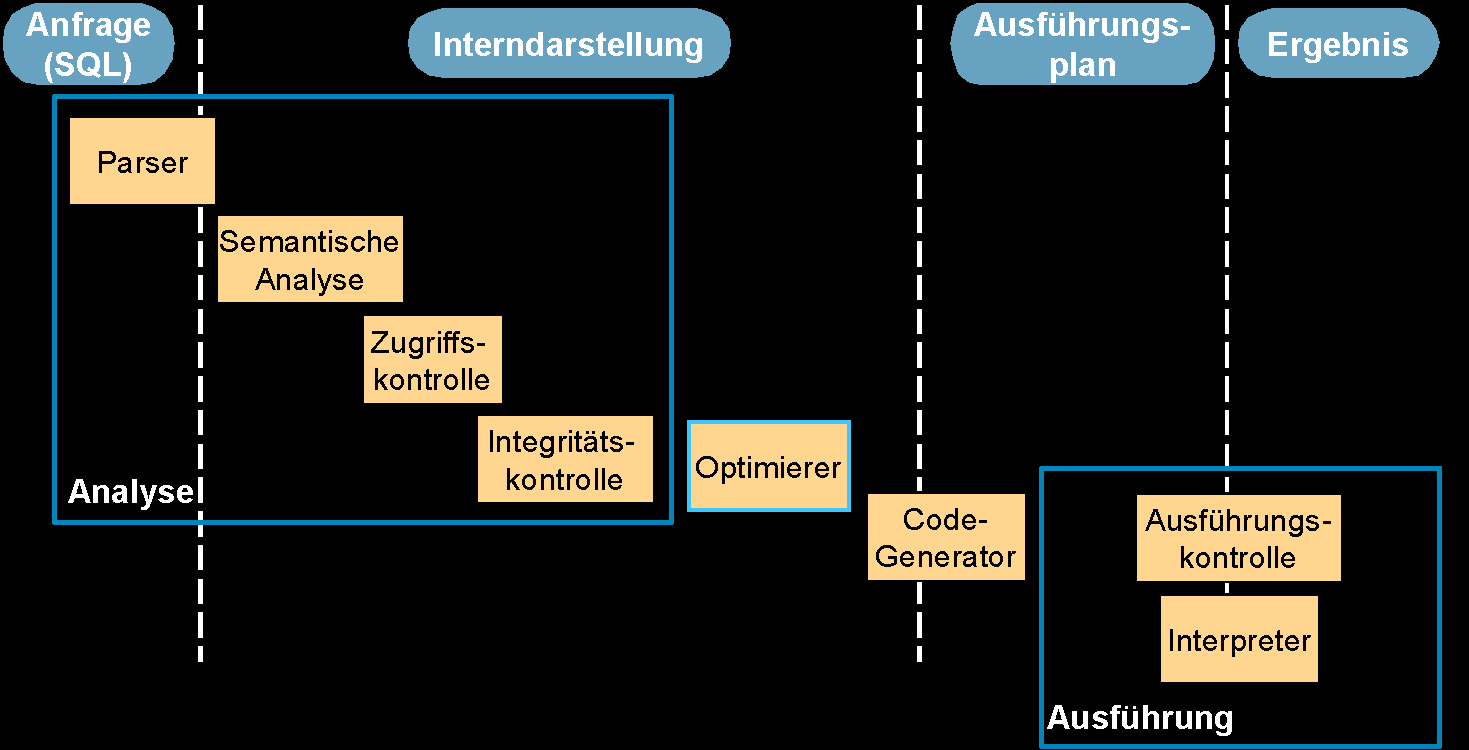
\includegraphics[width=1\linewidth]{Pictures/U10-Beamer-Anfrageverarbeitung}
\pagebreak
\end{beamerText}
